\subsection{Calcul de propriétés moléculaires}

\par Afin de pouvoir prédire les propriétés électroniques d'une molécule, les chimistes ont besoin de connaître avec une grande précision sa géométrie et certaines propriétés énergétiques. La connaissance précise de la position du nuage électronique d'une molécule dans ses différents niveaux d'énergie permet notamment de prédire les longueurs d'ondes absorbées pour un état d'énergie donné et émises lors du passage d'un état d'énergie à un autre, ce qui permet de prédire sa couleur.
De plus, la connaissance précise des nuages électroniques d'un couple de molécule dans leurs états fondamentaux et excités permet de prédire leur potentiel photovoltaïque. \\

\par Les nuages électroniques moléculaires sont exprimés mathématiquement à partir de fonctions d'ondes, qui sont l'approximation par la somme de fonctions gaussiennes de solutions d'équations dont la résolution analytique est impossible avec les outils mathématiques actuels. Le calcul de ces fonctions d'ondes est donc un enjeu fondamental en chimie, et est malheureusement très coûteux en termes de puissance et de temps de calcul. Le calcul de la fonction d'ondes d'une molécule de taille moyenne (environ 50 atomes) peut en effet prendre plusieurs semaines. \\

\par Dans la figure ci-dessous, on représente les iso-niveaux de probabilité de présence des électrons d'une molécule (nuage électronique), calculés à partir de sa fonction d'ondes. On considère que les surfaces de couleurs différentes représentent la même information.\\ 

\begin{figure}[!h]
	\centering
	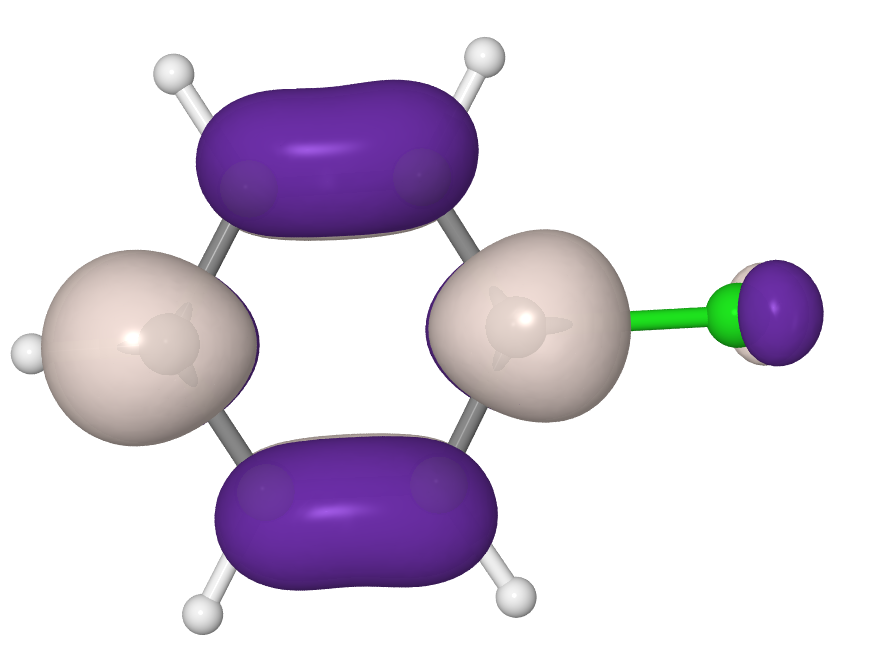
\includegraphics[scale=0.25]{images/iso_niveaux.png}
	\caption{Représentation des iso-niveaux de probabilité de présence électronique d'une molécule}
\end{figure}

\par Le calcul de la géométrie (position des atomes) et des propriétés énergétiques d'une molécule dépendent des fonctions d'ondes. Dans le cadre de ce stage, nous nous intéressons uniquement à la prédiction de géométries moléculaires optimisées (convergées), c'est pourquoi les deux parties suivantes vont décrire les approches actuellement utilisées en chimie pour calculer ces géométries. L'objectif de ces deux méthodes est de calculer une géométrie optimisée à partir d'une géométrie issue de mesures expérimentales ou de résultats théoriques.

\subsection{Mécanique moléculaire}
La mécanique moléculaire, à travers des outils comme OpenBabel\cite{openbabel} permet d'optimiser la géométrie des molécules selon des règles de distances typiques entre des couples d'atomes et d'angles typiques entre des liaisons. Il s'agit d'une approche simple qui ne permet pas d'obtenir une précision suffisante pour prédire les propriétés moléculaires. Du fait de sa rapidité, elle peut néanmoins être utilisée comme pré-traitement d'une géométrie théorique ou expérimentale et servir d'entrée à une optimisation géométrique quantique. 

\subsection{Optimisation géométrique quantique}
\par L'approche communément utilisée en chimie pour optimiser la géométrie moléculaire s'appuie sur l'optimisation itérative de la densité électronique. Elle est basée sur la \emph{Density Functional Theory} (DFT), qui propose une méthode dans laquelle la densité électronique d'une molécule est optimisée itérativement par la résolution d'équations, jusqu'à atteindre un seuil de cohérence donné. La géométrie moléculaire est alors déduite de la fonction d'onde, elle-même déduite de la densité électronique. Cette méthode est implémentée dans de nombreux programmes de chimie computationnelle, dont notamment Gaussian et Gamess.\\

\par L'inconvénient principal de cette approche est le temps de calcul nécessaire, qui limite la possibilité de l'appliquer à un grand nombre de molécules. Si l'on possédait une méthode plus rapide, on pourrait par exemple imaginer l'automatisation de la recherche de couples de molécules ayant un potentiel photovoltaïque élevé et dont la synthèse serait moins polluante que les couples utilisés actuellement, en associant à la recherche une fonction de coût qui représenterait le coût écologique de la synthèse.\\
Afin de réduire le temps d'optimisation, nous tentons de développer une solution basée sur l'élaboration de modèles d'apprentissage automatique, qui remplaceraient partiellement ou en totalité le calcul itératif de la fonction d'ondes.